% chktex-file 3
% chktex-file 13

\documentclass[11pt, letterpaper, twoside]{article}
\usepackage[utf8]{inputenc}
\usepackage[fleqn]{amsmath}
\usepackage[british]{babel}
\usepackage[T1]{fontenc}
\usepackage[inner=2.5cm, outer=2.5cm, top=3cm, bottom=3cm]{geometry}
\usepackage[hidelinks]{hyperref}
\usepackage{cancel}
\usepackage{cleveref}
\usepackage{aligned-overset}
\usepackage{booktabs}
\usepackage{textcomp}
\usepackage{changepage}
\usepackage[acronym,toc,nogroupskip,nopostdot,seeautonumberlist,nonumberlist]{glossaries}
\usepackage{upquote,textcomp}
\usepackage{subcaption}

\usepackage{pgfplots}
\pgfplotsset{compat=newest}
\usetikzlibrary{plotmarks}
\usetikzlibrary{arrows.meta}
\usepgfplotslibrary{patchplots}
\usepackage{grffile}

\graphicspath{ {./media/} }

\bibliographystyle{acm}

% \allowdisplaybreaks%

\title{Handover report}
\author{Martino Pilia}
\date{\today}

\newglossary[symg]{symbol}{syms}{symo}{Symbols}

\setglossarysection{section}
\makeglossaries%

\newacronym
    {vio}
    {VIO}
    {visual-inertial odometry}

\newacronym
    {slam}
    {SLAM}
    {simultaneous localisation and mapping}

\newacronym
    {sota}
    {SotA}
    {state-of-the-art}

\newacronym
    {ros}
    {ROS}
    {Robot Operating System}

\newacronym
    {rpc}
    {RPC}
    {remote procedure call}

\newacronym
    {lts}
    {LTS}
    {long-term support}

\newacronym
    {bow}
    {BoW}
    {bag-of-words}

\newacronym
    {ba}
    {BA}
    {bundle adjustment}

\newacronym
    {pnp}
    {PnP}
    {perspective-n-point}

\newacronym
    {spark}
    {SPARKlab}
    {Sensing, Perception, Autonomy, and Robot Kinetics laboratory}

\newacronym
    {rtabmap}
    {RTAB-Map}
    {Real-Time Appearance-Based Mapping}

\newacronym
    {introlab}
    {IntRoLab}
    {Intelligent Robot Lab}

\newacronym
    {rgbd}
    {RGB-D}
    {colour-depth}

\newacronym
    {imu}
    {IMU}
    {inertial measurement unit}

\newacronym
    {ir}
    {IR}
    {infrared}

\newacronym
    {sgm}
    {SGM}
    {semi-global matching}

\newacronym
    {fov}
    {FoV}
    {field of view}

\newacronym[
    plural=DoF,
    firstplural=degrees of freedom
    ]
    {dof}
    {DoF}
    {degree of freedom}

\newacronym
    {cde}
    {CDE}
    {code, data, and environment}

% \newacronym
%     {}
%     {}
%     {}


\begin{document}

\maketitle

\begin{abstract}
    This document is a brief report of activities performed between November 2019
    and January 2020, concerning the investigation of \gls{sota} tools
    for \gls{slam} based on \gls{vio}, meant to identify a suitable starting point
    to implement indoor localisation solutions on mobile devices.
\end{abstract}

\newpage

\tableofcontents

\newpage

\glsfindwidesttoplevelname[\acronymtype]
\printglossary[type=\acronymtype,style=alttree,title=Abbreviations,nonumberlist]

\newpage

\section{Introduction}

\subsection{Scope}

This document presents a preliminary evaluation of mapping and localisation
tools, aimed to explore the current \gls{sota} and to identify a suitable
starting point for further development of mobile localisation and mapping
applications.

\subsection{Tools and materials}

\subsubsection{The Robot Operating System}

\gls{ros}\footnote{\url{https://www.ros.org}} is a software framework
developed at Stanford University as a platform for robotic research. Despite
its name, it is not a true operating system, but rather a software framework
that runs as a set of applications on Linux, Windows, or Mac. \gls{ros} has a
modular design and allows to break a robotic system into multiple, re-usable
applications (e.g.\ controlling different sensors or actuators).

\gls{ros} applications can be distributed, built and installed as
\textit{packages} whose build system, catkin, is a collection of CMake macros.
Ros applications are executed as \textit{nodes}, communicating over the network
so they can effectively run over different physical units. \gls{ros} nodes
communicate by sending network packages through streams called \textit{topics},
and via an \gls{rpc} mechanism (known as \gls{ros} \textit{services}).

\gls{ros} is released in
\textit{distributions},\footnote{\url{http://wiki.ros.org/Distributions}} each
of those is supported on specific versions of Ubuntu. At the time of writing,
\gls{ros} 1.x is still the most widely used. \gls{ros} 2.x is a new generation
system, developed in parallel and largely incompatible with 1.x. In the
following, only \gls{ros} 1.x will be used.

A detailed introduction to the \gls{ros} is beyond the scope of the present
document, and comprehensive documentation and tutorials are available on the
official wiki.\footnote{\url{http://wiki.ros.org}} If not familiar with
\gls{ros}, a walk through the tutorials is highly
recommended.\footnote{\url{http://wiki.ros.org/ROS/Tutorials}}

\subsubsection{Kalibr}\label{sec:kalibr}

Kalibr is an open source tool developed at ETH Zürich for multi-camera,
multi-IMU, and camera-IMU
calibration.\footnote{\label{note:kalibr}\url{https://github.com/ethz-asl/kalibr}} Detailed
instructions and a video-tutorial can be found on the Kalibr
wiki.\footnote{\url{https://github.com/ethz-asl/kalibr/wiki}} The tool requires
\gls{ros} to build, however a \gls{ros}-free binary distribution is available
as a \gls{cde} package. Using \texttt{rosbag} is also the easiest way to
collect calibration data.

Kalibr supports different types of calibration target, including April grid,
circle grid, and checkerboard (the first is the most robust). When calibrating
the distortion coefficients, it is recommended to use a highly flat target
(e.g.\ printed on a rigid and flat plate).

\subsubsection{Intel RealSense}

Intel RealSense is a line of computer vision sensors aimed at robotics
applications. The current generation includes the RealSense D415 and
D435\footnote{A variant with 6 \gls{dof} \gls{imu} exists as D435i.} depth
cameras and the RealSense T265 tracking camera. A lidar sensor, the RealSense
L515, is planned to hit the market in April 2020. Previous generations include
the 3D cameras F200, S200, and SR300.

The RealSense SDK (\texttt{librealsense}) is available as open source
software,\footnote{\url{https://github.com/IntelRealSense/librealsense}} and a
broad documentation is provided by
Intel\footnote{\url{https://dev.intelrealsense.com/docs/docs-get-started}},
together with a collection of code samples (available in the GitHub repository)
and tutorials. The SDK allows to seamlessly integrate multiple RealSense
devices using a uniform API.

In the lab, a RealSense D435 and a T265 are available. The D435 is a depth
camera with one RGB and two \gls{ir} global shutter sensors (87\textdegree{}
\gls{fov}), that provide RGB and rectified grayscale stereo feeds (pinhole
distortion model, 50~mm baseline). The camera performs on-board computation of a
depth map by \gls{sgm}, and it is equipped with an \gls{ir} projector that
enhances the quality of the depth, especially in textureless
areas.\footnote{Since the \gls{ir} pattern creates spurious features in the
    image, care should be put to disable it when directly using the stereo
    images in some applications (e.g.\ feature-based stereo \gls{slam}).}

The T265 is a tracking camera equipped with a 6 \gls{dof} \gls{imu} and a
stereo pair of fisheye lens sensors (163\textdegree{} \gls{fov}, 65~mm
baseline). The camera implements an on-board visual-inertial \gls{slam} system
(with loop closure and relocalisation) and provides as output the 6D pose,
together with the raw streams for the two fisheye sensors, the gyroscope and
the accelerometer.\footnote{The T265 is not a depth camera, and while it is
    possible (on the host) to rectify the stereo images and compute a depth map
    from them, the quality of such depth map is significantly inferior to the
    depth camera. For an example of how to rectify fisheye images and perform
    stereo matching, see the example in the \texttt{librealsense} SDK:
\url{https://github.com/IntelRealSense/librealsense/blob/83f952a4bd/wrappers/python/examples/t265_stereo.py}}

The depth and tracking cameras can be combined together for 3D reconstruction
tasks. The 3D model of a support for both cameras is provided by
Intel,\footnote{\url{https://github.com/IntelRealSense/librealsense/tree/3b14a5c/examples/tracking-and-depth}}
together with a calibration
matrix,\footnote{\url{https://github.com/IntelRealSense/librealsense/blob/3b14a5c876/examples/tracking-and-depth/H_t265_d400.cfg}}
and a 3D-printed copy is already available in the lab.\footnote{Such support
    can then be mounted on a tripod, or it is possible to attach it to a
    laptop. For the latter use case, it is possible to 3D-print a fixture that
    can be taped to the lid of the laptop, and allows to attach and detach the
    camera support via its dove-tail joint. The STL file for such fixture is
    available at
\url{https://github.com/m-pilia/phd-handover-report/blob/master/data/fixture.stl}.}
A calibration of the rig can be performed with Kalibr (\cref{sec:kalibr}) if
necessary.

\subsubsection{MyntEye}

A MyntEye S 1030 stereo camera is available in the lab. It is equipped with two
global shutter fisheye lens sensors (122\textdegree\texttimes76\textdegree,
120~mm baseline), \gls{ir} projectors, and 6 \gls{dof} \gls{imu}. The SDK is
available as open source
software\footnote{\url{https://github.com/slightech/MYNT-EYE-S-SDK}} and
includes a \gls{ros}
wrapper.\footnote{\url{https://github.com/slightech/MYNT-EYE-S-SDK/tree/master/wrappers/ros}}

The camera is not self-calibrating, and calibration of the distortion
parameters needs to be performed manually with a tool provided by the
manufacturer.\footnote{\url{https://mynt-eye-s-sdk.readthedocs.io/en/2.3.9/src/tools/calibration_tool.html}}
Camera-IMU calibration can be performed with
Kalibr.\textsuperscript{\ref{note:kalibr}}

While the higher baseline should give this camera more range, the quality of
the depth map seems worse compared to the RealSense.\footnote{The camera
available in the lab is likely to require a new calibration of the intrinsics,
including the distortion coefficients.} The SDK and documentation are also less
mature.

\subsubsection{ZED camera}

The ZED camera\footnote{\url{https://www.stereolabs.com/zed/}} is a stereo
camera manufactured by ZED Labs. At Tampere University, some units are
available at CIVIT.

The API is fairly mature and exposes both access to the raw data (streams for
raw and rectified stereo images and depth map) and to high-level features such
as mapping and 3D scanning. The SDK is however proprietary, close source
software. Another noteworthy limitation is that the depth map is computed on
the host, and the SDK requires a CUDA-enabled Nvidia GPU to work.

\subsubsection{OpenVSLAM}

OpenVSLAM~\cite{openvslam2019} is a \gls{slam} system developed at the National
Institute of Advanced Science and Technology in Japan. It consists of a C++
library based on OpenCV that allows to perform \gls{slam} based on pure visual
odometry, and supports multiple camera configurations as input, including
monocular, stereo, and RGB-D, with several lens models (pinhole, fisheye,
equirectangular). While being very young, the project has good quality and
coding standards, and it is currently under active development.

Detailed usage examples are
provided,\footnote{\url{https://openvslam.readthedocs.io/en/master/example.html}}
ready to run on known benchmark datasets (such as Kitti~\cite{geiger2013vision}
or TUM-VI~\cite{schubert2018vidataset}) or user data (e.g.\ on a video file). A
Docker image and a \gls{ros} package are also provided by the authors.

OpenVSLAM provides fairly good visual odometry based on point matching, by
extracting ORB~\cite{rublee2011orb} corners in each frame. It implements loop
closure detection, based on a \gls{bow} model: loop closure candidates are
searched among frames containing a sufficiently high number of corresponding
visual words and are confirmed by geometric verification. If a suitable
candidate is found, a loop closure edge is added to the pose graph, that is in
turn optimised with g2o~\cite{grisetti2011g2o}. This mechanism works reasonably
in some environments, but it easily fails in presence of perceptual aliasing
(e.g.\ when navigating through similar corridors in an office space), due to
the lack of any mechanism to cope with outliers in the loop closure detection.

Localisation is also based on \gls{bow}, by retrieving a frame with similar
visual words and subsequently recovering the camera pose through \gls{pnp}.
This approach works on a single session \gls{slam}, but it is likely not robust
enough to handle localisation in multiple sessions with varying conditions
(illumination, crowding, etc.) or image data from different sensors.

While OpenVSLAM is reasonably optimised for speed, it is not optimised for
memory usage. The map can be stored to disk in messagepack format, to be
subsequently loaded in a new session, and it is kept in memory in a JSON
structure, as most other data structures in the software, therefore incurring
in a serious memory overhead. This is a limiting factor, making it impossible
to map a space significantly larger than Kampusareena when using a laptop with
32~GB of memory. Another limiting factor is the time required to perform
\gls{ba}, that grows without bounds with the size of the pose graph, requiring
several minutes to complete a loop closure on a map with a few thousand
keyframes.

\subsubsection{Kimera}

Kimera~\cite{rosinol2019kimera} is a software library for semantic \gls{slam}
implemented at the
\gls{spark}.\footnote{\url{https://github.com/MIT-SPARK/Kimera}} It is composed
of four modules:
\begin{itemize}
    \item
        Kimera-VIO,\footnote{\label{note:kimera_vio}\url{https://github.com/MIT-SPARK/Kimera-VIO}} a
        \gls{vio} library that implements the \gls{slam} frontend;
    \item
        Kimera-RPGO,\footnote{\url{https://github.com/MIT-SPARK/Kimera-RPGO}}
        a library based on GTSAM~\cite{dellaert2006square,dellaert2012factor}
        that implements pose graph optimisation for loop closures;
    \item
        Kimera-Mesher, a module that provides real-time mesh generation
        (implemented in the Kimera-VIO
        repository);\textsuperscript{\ref{note:kimera_vio}}
    \item
        Kimera-Semantics,\footnote{\url{https://github.com/MIT-SPARK/Kimera-Semantics}}
        a library that adds real-time semantic labels to the mesh.
\end{itemize}

The library can be used to implement a standalone SLAM system, and a \gls{ros}
package is provided by the
authors.\footnote{\url{https://github.com/MIT-SPARK/Kimera-VIO-ROS}}.

Kimera is a very young project and, at the time of writing, the code is not
stable nor close to being production-ready. The odometry seems to be working
but the loop closure integration in the \gls{slam} system seems to be currently
broken. While the code may not be practical to be directly reused, at least for
the moment, it is a noteworthy reference to previous work, especially with
respect to the integration of real-time semantics in a \gls{slam} system. It
also represents a real example of usage for GTSAM.

The pose graph optimisation in Kimera-RPGO implements robust loop closures on
top of GTSAM, with an outlier rejection mechanism~\cite{mangelson2018pairwise}.
Being separated from the rest of the system, it is possible to easily re-use it
as a building block for a different \gls{slam} solution, or use it as a
baseline for experiments on loop closure.

\subsubsection{RTAB-Map}

\gls{rtabmap}~\cite{labbe2019rtab} is a \gls{slam} framework developed at the
\gls{introlab}, Université de Sherbrooke. It is a mature and feature-rich
framework, under active development, that provides:
\begin{itemize}
    \item visual \gls{slam} based on \gls{rgbd}, stereo, or lidar input;
    \item multi-session mapping, built-in ability and tools to import,
        manipulate, and export maps;
    \item optimisation for mapping of large environments;
    \item built-in integration with several odometry front-ends;
    \item integration with several solvers for \gls{ba} and loop closure
        (ceres,\footnote{\url{http://ceres-solver.org/}}
        g2o~\cite{grisetti2011g2o}, GTSAM~\cite{dellaert2006square},
        cvsba\footnote{\url{https://www.uco.es/investiga/grupos/ava/node/39}}~\cite{lourakis2009sba});
    \item integration of switchable constraints~\cite{sunderhauf2012switchable}
        for robust loop closures
        (Vertigo\footnote{\url{https://openslam-org.github.io/vertigo.html}});
    \item out-of-the-box integration with several cameras, including ZED,
        RealSense, and Kinect;
    \item runs as a standalone GUI application or as a \gls{ros} node;
    \item tools for debug and introspection;
    \item a large number of options and tunable parameters;
\end{itemize}

Detailed documentation can be found on the GitHub
wiki\footnote{\url{https://github.com/introlab/rtabmap/wiki}} for the
standalone version and on the \gls{ros}
wiki\footnote{\url{http://wiki.ros.org/rtabmap_ros}} for the \gls{ros} package
(\texttt{rtabmap\_ros}).

Pre-built binaries for both the standalone application and for the \gls{ros}
package are available in the \gls{ros} Ubuntu repository, however the pre-built
version is missing several optional components (e.g.~integration with GTSAM or
RealSense). It is possible to check what components are built in the current
version by running \texttt{rtabmap -{}-version}, and to enable more components
it is necessary to build \gls{rtabmap} from source, after installing or
building the desired components and making sure that the respective packages
are detected by CMake.

Besides of the aforementioned documentation, further examples of usage are
provided on the \gls{ros}
wiki\footnote{\url{http://wiki.ros.org/rtabmap_ros/Tutorials/HandHeldMapping}}
and on the RealSense
wiki\footnote{\url{https://github.com/IntelRealSense/realsense-ros/wiki/SLAM-with-D435i}}.
The latter example shows how perform sensor fusion with an external library
(using the \texttt{robot\_localization}
package)\footnote{\url{http://wiki.ros.org/robot_localization}} to compute the
\gls{vio} externally and feed the resulting odometry to \gls{rtabmap}.

\section{Experiments}

\subsection{Environment}

The experiments were conducted on a Lenovo ThinkPad T480 laptop equipped with
an Intel i7--8650U CPU and 32~GB of memory. Tests were conducted both on Arch
Linux and Ubuntu 16.04. The following instructions allow to reproduce the
experimental environment on Ubuntu 16.04 or 18.04.

\begin{enumerate}

    \item A clean environment on Ubuntu 16.04 (Xenial) or 18.04 (Bionic) is
        assumed. In this work, a fresh installation of Ubuntu 16.04.6 was used.

        The \texttt{realsense-ros} package is officially supported only on
        \gls{ros} kinetic on Ubuntu 16.04, but it seems to work on \gls{ros}
        melodic on Ubuntu 18.04 as well, as long as the \gls{lts} Linux kernel
        is used (version 4.15, provided by the apt package
        \texttt{linux-generic}). If replicating the results on Ubuntu 18.04, it
        is necessary to replace Xenial with Bionic and \texttt{ros-kinetic}
        with \texttt{ros-melodic} in the following instructions.

    \item (Optional) While not strictly necessary, it is recommended to install
        ccache, since it can greatly speeds up repeated builds.
\begin{verbatim}
sudo apt-get install -y ccache
sudo /usr/sbin/update-ccache-symlinks
echo 'export PATH="/usr/lib/ccache:$PATH"' > ~/.bashrc
source ~/.bashrc
\end{verbatim}

    \item Install \gls{ros} Kinetic from the \gls{ros} deb repository,
        following the upstream instruction on the
        wiki.\footnote{\url{http://wiki.ros.org/kinetic/Installation/Ubuntu}}

    \item Install the \texttt{ros-kinetic-rqt-configure} package with
        \texttt{apt}. This tool is not strictly necessary, but it is useful to
        quickly inspect and change \gls{ros} parameters. Make sure that the
        tool correctly works by launching it with
\begin{verbatim}
rosrun rqt_configure rqt_configure
\end{verbatim}
        (a \texttt{roscore} instance needs to be running: if you are not sure
        what this means, a walk through the \gls{ros} tutorials is recommended
        before continuing).

    \item Install \texttt{librealsense} from the Intel deb repository,
        following the upstream instructions on
        GitHub.\footnote{\url{https://github.com/IntelRealSense/librealsense/blob/e8cb6b4/doc/distribution_linux.md\#installing-the-packages}}
        In this work, \texttt{librealsense} 1.32.0 was used.

        After the installation, connect the RealSense devices, launch
        \texttt{realsense-viewer}, and make sure that they are working
        correctly. Ensure that the depth map and the stereo images are received
        at the correct frame rate, stuttering or flickering can be symptoms of
        low level problems (e.g.\ issues with the kernel modules, or
        insufficient bandwidth on the USB controller).

    \item Install \texttt{realsense-ros}. At the time of writing, this package
        is not available as a binary distribution and needs to be built from
        source. Create a catkin workspace and build it by following the
        upstream instructions on
        GitHub.\footnote{\url{https://github.com/IntelRealSense/realsense-ros/blob/69d199d/README.md\#step-3-install-intel-realsense-ros-from-sources}}
        In this work, \texttt{realsense-ros} 2.2.12 was used.

        The workspace needs to be enabled in the shell when working with the
        cameras. The following command (from the aforementioned instructions)
        automatically enables it within any bash session:
\begin{verbatim}
echo "source ~/catkin_ws/devel/setup.bash" >> ~/.bashrc
\end{verbatim}
        After the installation, make sure that \texttt{realsense-ros} is
        correctly working by running one of the example launchfiles, for
        instance the point cloud publisher\footnote{\url{https://github.com/IntelRealSense/realsense-ros/blob/69d199d/README.md\#rgbd-point-cloud}}
\begin{verbatim}
roslaunch realsense2_camera rs_camera.launch filters:=pointcloud
\end{verbatim}
        and in another shell launch \texttt{rviz} to display the point cloud.
        In \texttt{rviz}, under the tree view displayed in the panel on the
        left dock, set the \texttt{Fixed frame} (under \texttt{Global Options})
        to \texttt{camera\_link}, and enable the point cloud by clicking the
        \texttt{Add} button on the bottom left, in the dialog window switch to
        the \texttt{By topic} tab, and select the \texttt{pointcloud2} topic
        (under \texttt{depth\_registered/points}).\footnote{To get familiar
        with \texttt{rviz}, a set of tutorials is available in the \gls{ros}
        wiki at \url{http://wiki.ros.org/rviz/Tutorials}.}

    \item Install \gls{rtabmap} and its \gls{ros} wrapper. The binary version
        from the \gls{ros} deb repository includes support for g2o and Vertigo,
        and was used in the experiments
\begin{verbatim}
sudo apt-get install ros-kinetic-rtabmap ros-kinetic-rtabmap-ros
\end{verbatim}

        Launch \texttt{rtabmap}, and if the installation was successful the GUI
        should open.

    \item (Optional) Some additional solvers (e.g.\ GTSAM, cvsba) and camera
        modules (e.g.\ to use RealSense devices from the standalone
        application) require to build \gls{rtabmap} from source, following
        upstream
        instructions.\footnote{\url{https://github.com/introlab/rtabmap_ros/blob/5b3fe2f/README.md\#build-from-source}}
        Before building from source, uninstall any existing \gls{rtabmap}
        binary packages from the system, to avoid unintentionally linking to
        the wrong libraries.

        When generating the build files with CMake (before
        running \texttt{make}), ensure that the desired components have been
        detected by CMake and are included in the build, by either inspecting
        the CMake console output or by opening the CMake cache and ensuring
        that the variable \texttt{WITH\_XXX} is set to \texttt{ON} (where
        \texttt{XXX} is the desired component, e.g.\ \texttt{GTSAM} or
        \texttt{CVSBA}).

    \item Install OpenCV 3.4 from source, following the upstream instructions
        in the OpenVSLAM
        documentation.\footnote{\url{https://openvslam.readthedocs.io/en/master/installation.html}}

    \item Install the
        MYNT-EYE-S-SDK.\footnote{\url{https://github.com/slightech/MYNT-EYE-S-SDK}}
        The SDK is available both as pre-build deb package or source
        distribution. It is recommended to build it from source, in order to
        avoid binary conflicts due to different versions of OpenCV, following
        upstream
        instructions.\footnote{\url{https://mynt-eye-s-sdk.readthedocs.io/en/latest/src/sdk/install_ubuntu_src.html}}

    \item Install the MYNT-EYE-S-SDK \gls{ros} wrapper, following upstream
        instructions.\footnote{\url{https://github.com/slightech/MYNT-EYE-S-SDK/tree/master/wrappers/ros}}

    \item (Optional) Install the ZED SDK following upstream
        instructions.\footnote{\url{https://www.stereolabs.com/developers/release/}}
        This is only required in order to use the ZED camera, and requires a
        CUDA-enabled Nvidia GPU available on the host.

\end{enumerate}

\subsection{Mapping with OpenVSLAM}

OpenVSLAM was tested as a front-end for real-time mapping with the ZED, MYNT,
and RealSense (both D435 and T265) cameras. In order to perform SLAM in
real-time, a small application was implemented, together with an abstract
interface that allows to use the four cameras. Source code and instructions are
available on GitHub.\footnote{\url{https://github.com/m-pilia/openvslam-example}}

Note that this application is not production-quality code, but rather a fast
prototype. It is lacking quality, features, and testing, and it was not
designed with the idea of being published.

\subsubsection{Build}

The following instructions allow to reproduce the environment on Ubuntu 16.04
or 18.04:\footnote{The repository has a continuous integration setup,
performing cloud builds inside a Docker container. It is possible to check
the Dockerfile located in the root of the repository to see a working
example of build environment on Ubuntu.}
\begin{enumerate}
    \item (Only on Ubuntu 16.04) Install an up-to-date version of CMake with
        support for C++17 (the default version 3.1 shipped with Ubuntu 16.04
        does not provide it).
\begin{verbatim}
wget -O - https://apt.kitware.com/keys/kitware-archive-latest.asc 2>/dev/null \
    | sudo apt-key add -
sudo apt-add-repository 'deb https://apt.kitware.com/ubuntu/ xenial main'
sudo apt-get update
sudo apt-get install -y cmake
\end{verbatim}

    \item (Only on Ubuntu 16.04) Install a more recent version of gcc, since
        the one shipped with Ubuntu 16.04 (gcc 5.4) does not have full support
        for C++17.
\begin{verbatim}
sudo add-apt-repository ppa:ubuntu-toolchain-r/test
sudo apt-get update
sudo apt-get install -y gcc-7 g++-7
[ ! -f /usr/sbin/update-ccache-symlinks ] || sudo /usr/sbin/update-ccache-symlinks
\end{verbatim}

    \item Build and install the OpenVSLAM library and its dependencies,
        following upstream
        instructions.\footnote{\url{https://openvslam.readthedocs.io/en/master/installation.html}}
        Note that OpenCV should already be installed if the environment setup
        instructions were followed. After building OpenVSLAM, install it by
        running \texttt{sudo make install} in the OpenVSLAM build
        folder.\footnote{If you prefer, you can install it in a local folder
        with \texttt{make DESTDIR=/some/local/folder install}; in that
        case, remember to pass \texttt{openvslam\_DIR=/some/local/folder}
        to CMake later, when building the \texttt{openvslam-example}
        repository.} In these tests, OpenVSLAM up to commit \texttt{f2945209fc} was
        used.

    \item Build the \texttt{openvslam-example} application. By default, support
        for RealSense and MYNT is built. It is possible to optionally build
        support for the ZED camera. The ZED module is however untested in its
        current state and may not work as intended.
\begin{verbatim}
git clone https://github.com/m-pilia/openvslam-example
cd openvslam-example
mkdir build && cd build

cmake .. # To build ZED support, use: cmake .. -DCAMERA_SLAM_WITH_ZED=ON
make -j"$(nproc)$"
\end{verbatim}

\end{enumerate}

\subsubsection{Usage}

The build procedure will produce a \texttt{camera\_slam} executable. To see the
available parameters:
\begin{verbatim}
    ./camera_slam --help
\end{verbatim}

Running a \gls{slam} mapping session requires to provide a destination for the
output map file, an ORB vocabulary,\footnote{A pre-built vocabulary can be
downloaded from the OpenVSLAM project at
\url{https://openvslam.readthedocs.io/en/master/simple_tutorial.html}.} and a
configuration file. Example configuration files are provided in the
\texttt{param} folder in the repository.

\begin{verbatim}
./camera_slam \
    -m RealSense \
    -c ./param/realsense_stereo.yaml \
    -v /path/to/the/orb/vocabulary \
    -output-map-db map.msg
\end{verbatim}

If everything works correctly, a couple of windows should open, showing the
pose graph and the current frame respectively (\cref{fig:openvslam_mapping}).

\begin{figure}[tb]
    \centering
    \begin{subfigure}[t]{.49\textwidth}
        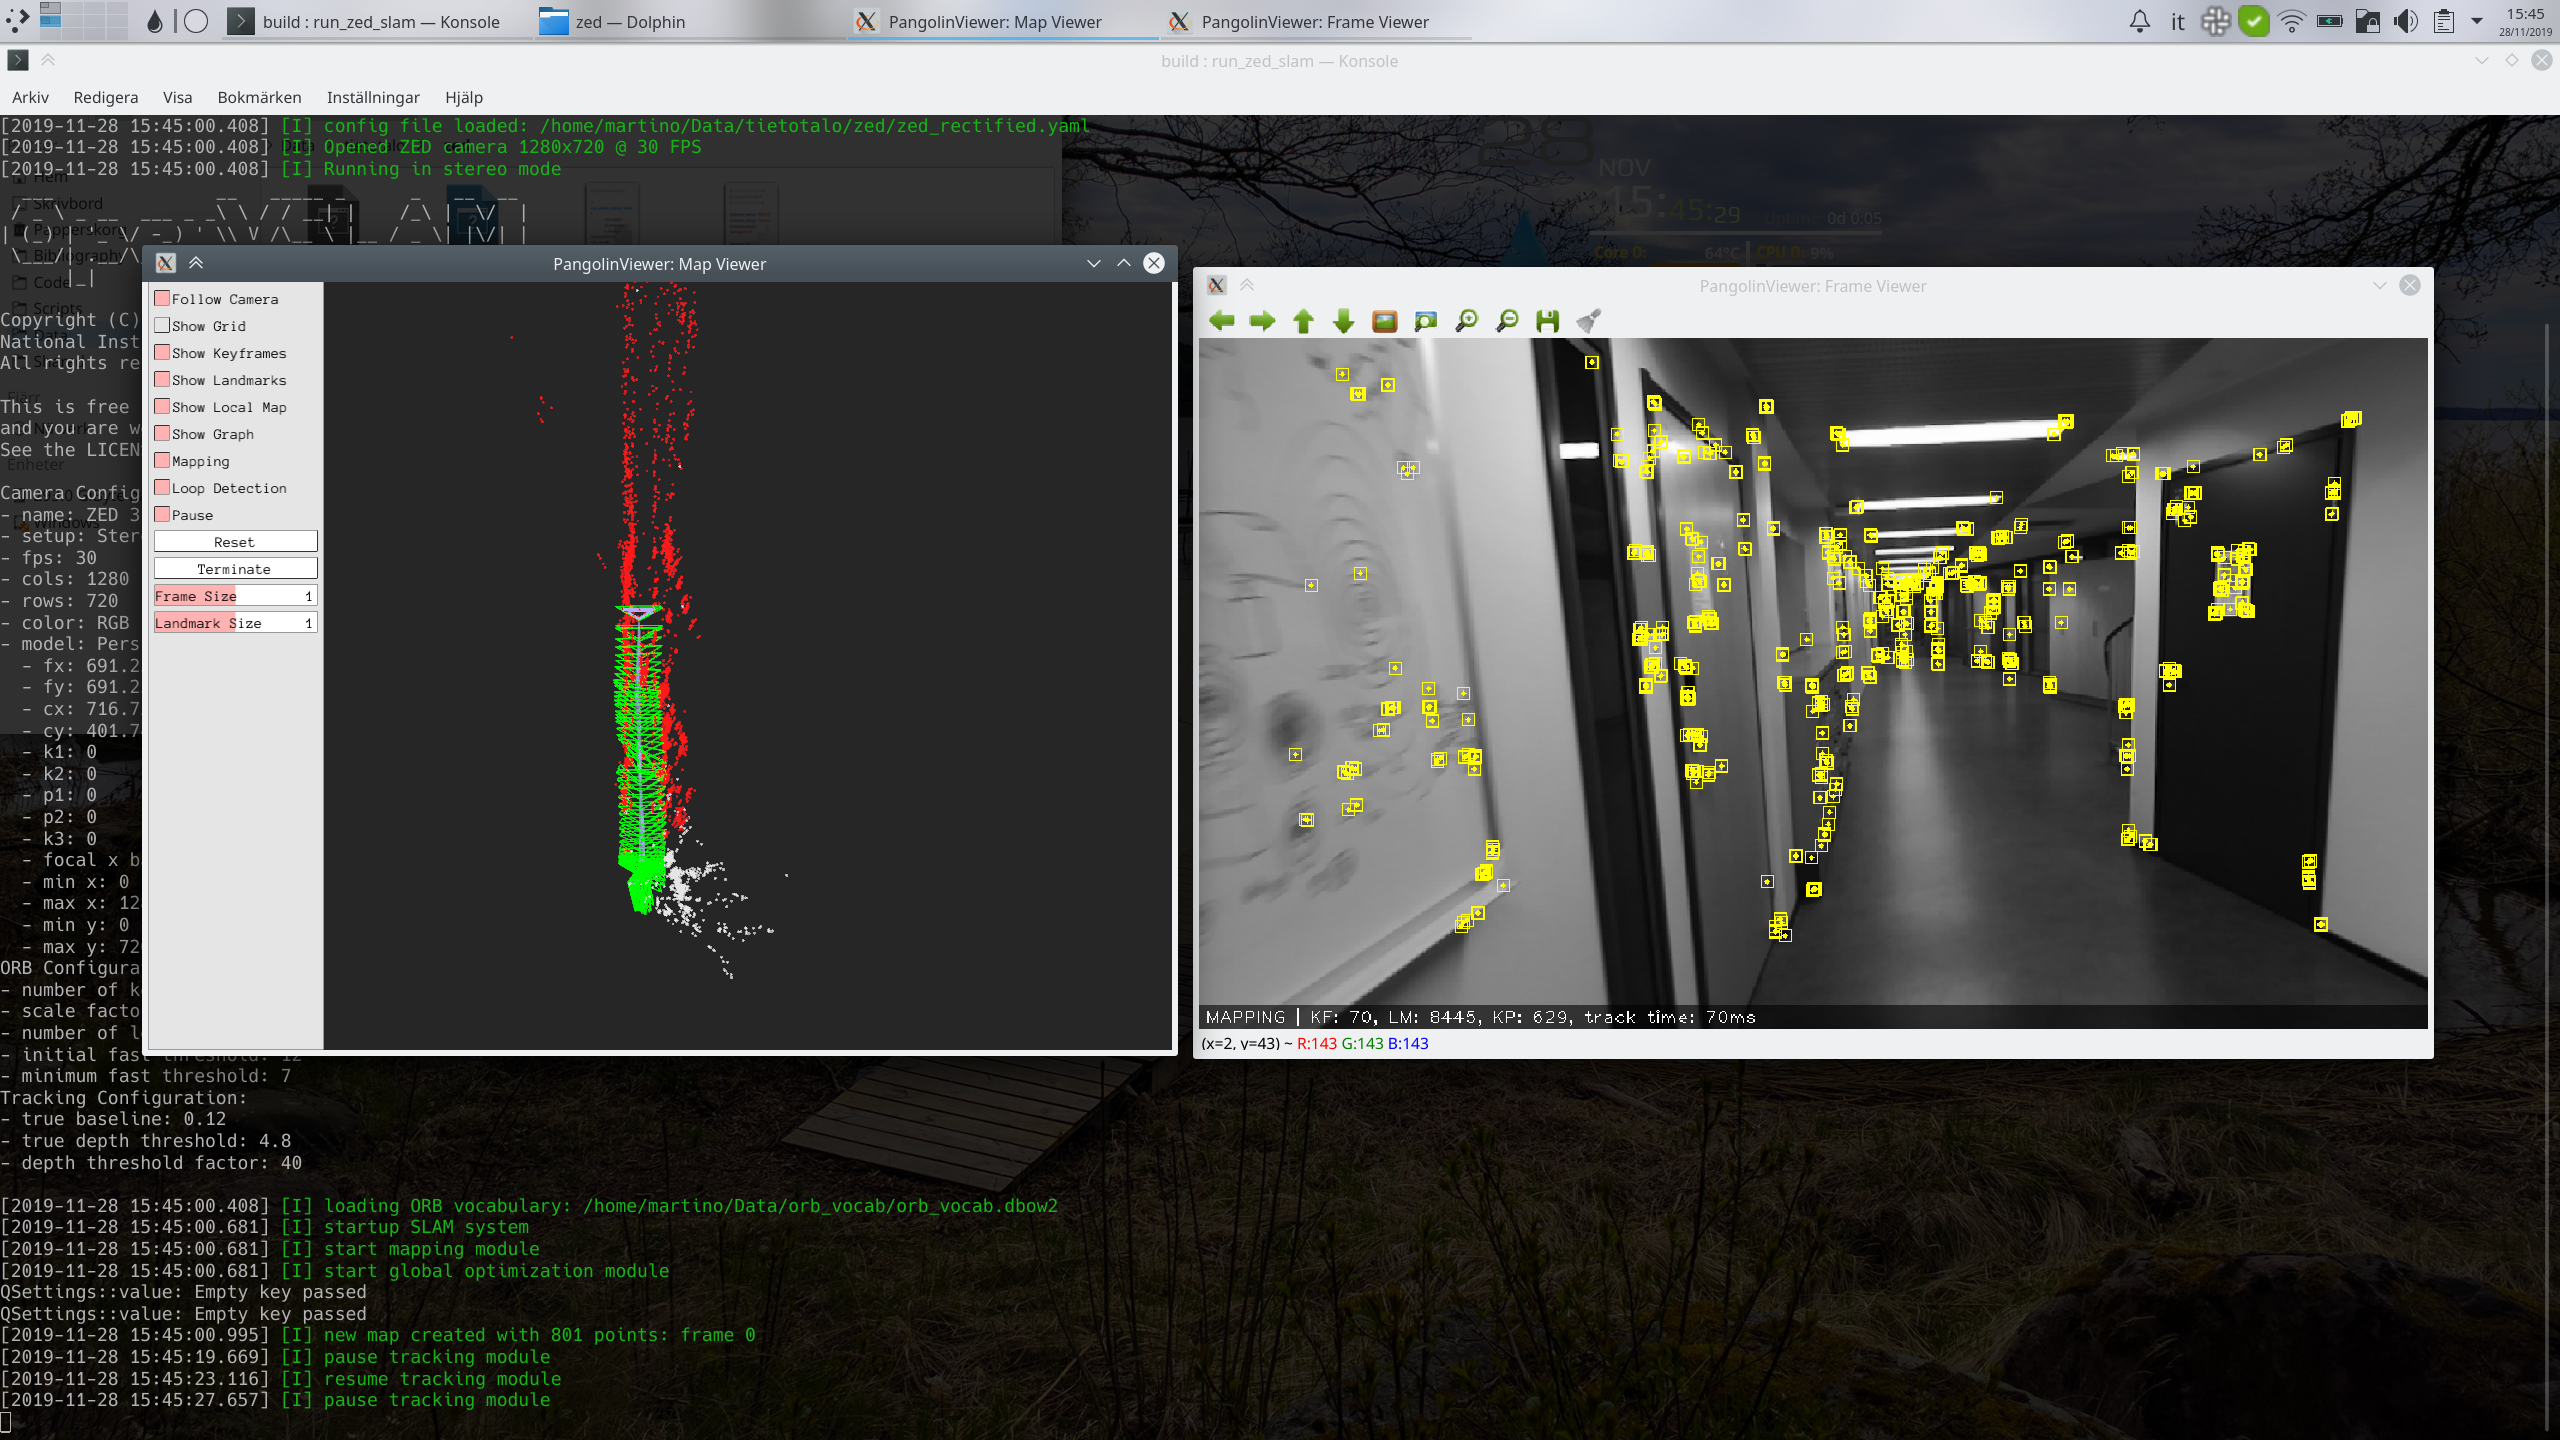
\includegraphics[width=\linewidth]{openvslam.png}
        \caption{Example mapping session.}\label{fig:openvslam_mapping}
    \end{subfigure}
    \begin{subfigure}[t]{.49\textwidth}
        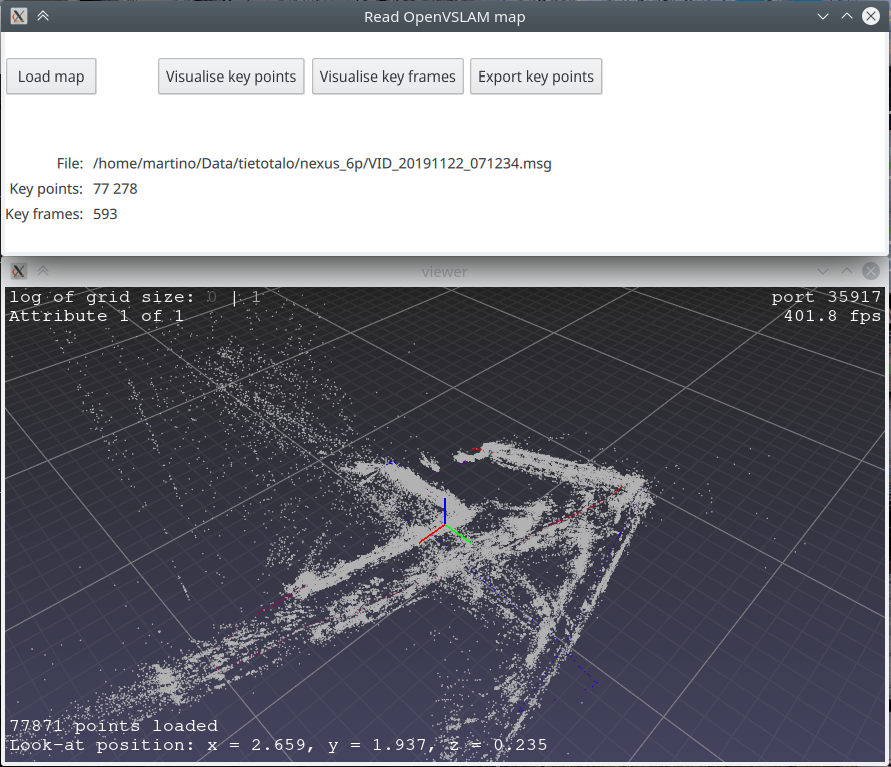
\includegraphics[width=\linewidth]{load_map.png}
        \caption{Example point cloud visualisation.}\label{fig:openvslam_load_map}
    \end{subfigure}
    \caption{Example of OpenVSLAM usage.}\label{fig:openvslam}
\end{figure}

\begin{figure}[h!]
    \centering
\end{figure}

To run a pure localisation session, it is necessary to load a pre-built map:

\begin{verbatim}
./camera_slam \
    --localization \
    -m RealSense \
    -c ./param/realsense_stereo.yaml \
    -v /path/to/the/orb/vocabulary \
    -input-map-db map.msg
\end{verbatim}

The \texttt{-{}-output-video} and \texttt{-{}-input-video} flags allow to
record and playback input data from file respectively. The output format
depends on the camera used (SVO for the ZED camera, \gls{ros} bagfile for the
ReRealSense, and a custom binary dump for the MYNT EYE\footnote{At the time of
writing, the MYNT EYE does not provide a raw data record and playback API,
so a very simplified mechanism was implemented in this repository.}).

The map is stored by OpenVSLAM as a messagepack dump (i.e.\ binary compressed
JSON), storing keypoints with descriptors and keyframes with pose graph. A
simple Python tool is provided in the repository in order to inspect the map
(\cref{fig:openvslam_load_map}).

\begin{verbatim}
# Install dependencies (example on Ubuntu 16.04)
apt-get update -y
apt-get install -y --no-install-recommends python3 python3-pip python3-pyqt5 \
    python3-pyqt5.qtopengl python3-pyqt5.qtquick python3-setuptools python3-venv \
    qml-module-* qmlscene

# Setup virtual environment
python3 -m venv ./scripts/.venv
source ./scripts/.venv/bin/activate
pip install -r ./scripts/requirements.txt

# run the tool
python ./scripts/read_map.py
\end{verbatim}

\subsubsection{Results}

\bibliography{bibliography}

\end{document}
